Up to this point, we have always made the assumption that one product (either raw material or temporary product) can only be used to build one, and only one, other product. In terms of BoM, this meant that every node (product) had at most one successor. In this new chapter, we will drop this assumption and examine how we can deal with this situation. From now on, we allow one node to have more than one successor.

\section{Adapting the $n_{if}$ coefficient}

Let's consider figure (\ref{shared_temp:basic_bom}) in which we have a product $i$ required to make three other temporary products. Up to now, we always considered that there was one path from $i$ to the final product $f$ so that \[ n_{if} = \prod_{(k,j)\in Path_{i\rightarrow f}}n_{kj} \] However, now, the notiton of $Path_{i\rightarrow f}$ becomes ambiguous. 

\begin{figure}[h!]
    \centering
    \subfigure{
    \subfigure{
        \begin{tikzpicture}
            \draw (0,0) node[draw, circle] (f) {$f$};
            \draw (-2, -2) node[draw, circle] (1) {$1$};
            \draw (2, -2) node[draw, circle] (2) {$2$};
            \draw (0, -4) node[draw, circle] (3) {$3$};
            \draw (-2, -6) node[draw, circle] (i) {$i$};
            \draw (2, -6) node[draw, circle] (4) {\vphantom{$f$}};

            \draw[->] (1) -- (f);
            \draw[->] (2) -- node[right] {$3$} (f);
            \draw[->] (3) -- node[left] {$2$} (1);
            \draw[->] (3) -- node[left] {$3$} (2);
            \draw[->] (i) -- (3);
            \draw[->] (i) -- (1);
            \draw[->] (4) -- (3);
            \draw[decorate, decoration={brace, amplitude=10pt}] (-5, -7) -- (5, -7);
        \end{tikzpicture}
    }

    \subfigure{
        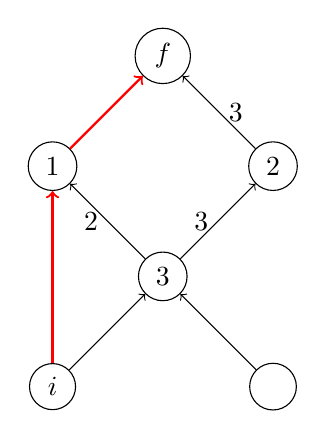
\begin{tikzpicture}[scale=.7]
            \draw (0,0) node[draw, circle] (f) {$f$};
            \draw (-2, -2) node[draw, circle] (1) {$1$};
            \draw (2, -2) node[draw, circle] (2) {$2$};
            \draw (0, -4) node[draw, circle] (3) {$3$};
            \draw (-2, -6) node[draw, circle] (i) {$i$};
            \draw (2, -6) node[draw, circle] (4) {\vphantom{$f$}};

            \draw[->, red, thick] (1) -- (f);
            \draw[->] (2) -- node[right] {$3$} (f);
            \draw[->] (3) -- node[left] {$2$} (1);
            \draw[->] (3) -- node[left] {$3$} (2);
            \draw[->] (i) -- (3);
            \draw[->, red, thick] (i) -- (1);
            \draw[->] (4) -- (3);
        \end{tikzpicture}
    }
    \subfigure{
        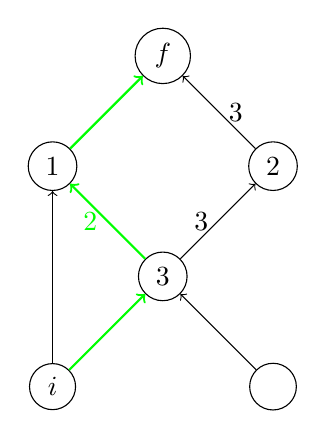
\begin{tikzpicture}[scale=.7]
            \draw (0,0) node[draw, circle] (f) {$f$};
            \draw (-2, -2) node[draw, circle] (1) {$1$};
            \draw (2, -2) node[draw, circle] (2) {$2$};
            \draw (0, -4) node[draw, circle] (3) {$3$};
            \draw (-2, -6) node[draw, circle] (i) {$i$};
            \draw (2, -6) node[draw, circle] (4) {\vphantom{$f$}};

            \draw[->, green, thick] (1) -- (f);
            \draw[->] (2) -- node[right] {$3$} (f);
            \draw[->, green, thick] (3) -- node[left] {$2$} (1);
            \draw[->] (3) -- node[left] {$3$} (2);
            \draw[->, green, thick] (i) -- (3);
            \draw[->] (i) -- (1);
            \draw[->] (4) -- (3);
        \end{tikzpicture}
    }
    \subfigure{
        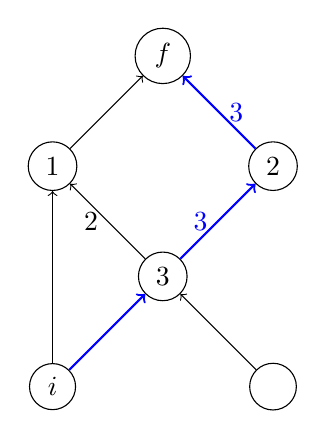
\begin{tikzpicture}[scale=.7]
            \draw (0,0) node[draw, circle] (f) {$f$};
            \draw (-2, -2) node[draw, circle] (1) {$1$};
            \draw (2, -2) node[draw, circle] (2) {$2$};
            \draw (0, -4) node[draw, circle] (3) {$3$};
            \draw (-2, -6) node[draw, circle] (i) {$i$};
            \draw (2, -6) node[draw, circle] (4) {\vphantom{$f$}};

            \draw[->] (1) -- (f);
            \draw[->, blue, thick] (2) -- node[right] {$3$} (f);
            \draw[->] (3) -- node[left] {$2$} (1);
            \draw[->, blue, thick] (3) -- node[left] {$3$} (2);
            \draw[->, blue, thick] (i) -- (3);
            \draw[->] (i) -- (1);
            \draw[->] (4) -- (3);
        \end{tikzpicture}
    }
    }
    \caption{\label{shared_temp:basic_bom}Dropping the unique path assumption}
\end{figure}% this is badly managed in the sense that if the page is re-dimensioned, the figure may fail to present accordingly... :( one solution to ensure its positioning would be something like minipage

But we can still reason about the bill of material and notice that the number of items $i$ needed to produce one item $f$ must take into account the number of items $i$ needed to produce the three temporary produce needed for $f$. Thus, the number of items $i$ needed is the sum between all the paths from $i$ to $f$ available in the bill of material. This property can be thought as a "superposition effect" typical in phisical systems. Finally, the following formula holds: \[ n_{if} = \sum_{ p \in\mathcal P(i,f)} n_{ij}^p \] where $\mathcal P(i,f)$ denotes the set of paths going from $i$ to $f$ and $n_{if}^p = \prod_{(k,j)\in p}n_{kj}$. 

Concerning figure (\ref{shared_temp:basic_bom}), we can see that there are three different paths from $i$ to $f$. Thus, it holds that
\[
    \begin{cases}
        n_{if}^{red} &= 1.1 = 1 \\
        n_{if}^{blue} &= 1.2.1 = 2 \\
        n_{if}^{green} &= 1.3.3=  9 \\
    \end{cases}
    \Rightarrow
    n_{if} = 2 + 1 + 9 = 12
\]

\section{A fully worked example}

In this section, we will treat a whole example using this new assumption. The example considered is associated to the bill of material represented in figure (\ref{shared_temp:bom}). 

\begin{figure}[h!]
    \centering
    \begin{tikzpicture}[xscale=.66]
        \draw (0,0) node[circle, draw] (f) {$f$};
        \opVal{0}{0}{$(1,1)$}
        \draw (-2, -2) node[circle, draw] (1) {$1$};
        \opVal{-2}{-2}{$(4,2)$}
        \draw (2, -2) node[circle, draw] (2) {$2$};
        \opVal{2}{-2}{$(2,2)$}
        \draw (-4, -4) node[circle, draw] (3) {$3$};
        \opVal{-4}{-4}{$(1,1)$}
        \draw (0, -4) node[circle, draw] (4) {$4$};
        \opVal{0}{-4}{$(1,5)$}
        \draw (4, -4) node[circle, draw] (RM1) {\vphantom{$f$}};
        \draw (-6, -6) node[circle, draw] (RM2) {\vphantom{$f$}};
        \draw (-2, -6) node[circle, draw] (5) {$5$};
        \opVal{-2}{-6}{$(3,3)$}
        \draw (2, -6) node[circle, draw] (6) {$6$};
        \opVal{2}{-6}{$(1,1)$}
        \draw (-2, -8) node[circle, draw] (RM3) {\vphantom{$f$}};
        \draw (2, -8) node[circle, draw] (7) {$7$};
        \opVal{2}{-8}{$(1,1)$}
        \draw (2, -10) node[circle, draw] (RM4) {\vphantom{$f$}};

        \draw[->] (1) -- (f);
        \draw[->] (2) -- (f);
        \draw[->] (3) -- (1);
        \draw[->] (4) -- (1);
        \draw[->] (4) -- (2);
        \draw[->] (RM1) -- (2);
        \draw[->] (RM2) -- (3);
        \draw[->] (5) -- (3);
        \draw[->] (5) -- (4);
        \draw[->] (6) -- (4);
        \draw[->] (7) -- (6);
        \draw[->] (RM4) -- (7);
        \draw[->] (RM3) -- (5);
    \end{tikzpicture}
    \caption{\label{shared_temp:bom}Bill of material for the worked example}
\end{figure}

Let's first begin by computing the different $n_{if}, \forall i$ taking into account every possible paths. Remember that when no $n_{ij}$ coefficient is written in the bill of material, it implies $n_{ij} = 1$. Hence the following results which can be found easily : 
\begin{align*}
    n_{ff} &= 1 & n_{1f} &= 1 & n_{2f} &= 1 & n_{3f} &= 1 \\
    n_{4f} &= 1+1 = 2 & n_{5f} &= 1+1+1 = 3 & n_{6f} &= 1+1=2 & n_{7f} &= 1+1 = 2
\end{align*}
As usual, the maximum production rate is given by the following 
\[
    \begin{split}
    X_f^{max}(b_f) &= \min_i\left( \frac{b_f}{T_{si} + T_{oi}b_fn_{if}} \right) \\
    &=
    \min\left(
        \frac{b_f}{1+b_f} ; 
        \frac{b_f}{4+2.b_f} ; 
        \frac{b_f}{2+2.b_f} ; 
        \frac{b_f}{1+b_f} ; 
        \frac{b_f}{2+5.2.b_f} ; 
        \frac{b_f}{3+3.3.b_f} ; 
        \frac{b_f}{1+1.2.b_f} ; 
        \frac{b_f}{1+2.b_f}
    \right)\\
    & \overset{b_f\rightarrow\infty}{=}
    \frac{1}{10}
    \end{split}
\]
Let's assume to produce at a rate $X_f^* = \frac{1}{11}$, what is the minimum batch size we can use ? Again, as usual, we compute it as the following
\begin{align*}
    b_f^* &= \max_i\left( \frac{X_f^*T_{si}}{1-X_f^*T_{oi}n_{if}} \right)\\
    &= \max\left(
        \frac{ \frac{1}{11}.1 }{ 1 - \frac{1}{11}.1 } ;
        \frac{ \frac{1}{11}.4 }{ 1 - \frac{1}{11}.2.1 } ;
        \frac{ \frac{1}{11}.2 }{ 1 - \frac{1}{11}.2.1 } ;
        \frac{ \frac{1}{11}.1 }{ 1 - \frac{1}{11}.1.1 } ;
        \frac{ \frac{1}{11}.2 }{ 1 - \frac{1}{11}.5.2 } ;
        \frac{ \frac{1}{11}.3 }{ 1 - \frac{1}{11}.3.3 } ;
        \frac{ \frac{1}{11}.1 }{ 1 - \frac{1}{11}.1.2 } ;
        \frac{ \frac{1}{11}.1 }{ 1 - \frac{1}{11}.1.2 }
    \right)\\
    &= 2
\end{align*}
Which means that producing at rate $\frac{1}{11}$ implies using a batch of at least $2$ items $f$. If we use such a batch size, the bottleneck machine would be machine $4$. Let's try to depict the GANT diagram.

The way of drawing the GANT diagram is the following : 
\begin{enumerate}
    \item Draw a repeatable GANT diagram taking into account the production time of each batch
    \item Identify the "schedule" for producing the first batch
    \begin{enumerate}
        \item Color the "boxes" associated to the machines without predecessors in the bill of material (these machines are the first (and only) machines to work during the first time window)
        \item In the subsequent time window, color the "boxes" associated to successors of machines for which associated box is already colored in the previous time window.
    \end{enumerate}
\end{enumerate}

Note that, still like before, it takes $L.D$ (where $L$ is the number of levels of bill of material) to produce the first batch. In our case, $D=b_f/X_f=22$. The associated GANT diagram is represented in figure (\ref{shared_temp:gant}).

\begin{figure}
    \begin{tikzpicture}[xscale=.15]
        \draw[->] (-2,0) node[left] {$f$} -- (5*22 + 2, 0);
        \foreach \y in {1,...,7} \draw[->] (-2, - \y) node[left] {$\y$} -- (5*22 + 2, -\y);

        \foreach \d\y\t in {0/5/21, 0/7/5, 1/3/3, 1/6/5, 2/4/22, 3/1/8, 3/2/6, 4/0/3} {
            \draw[pattern=north west lines, pattern color=black!30!green] (\d * 22, -\y) rectangle (\d * 22 + \t, -\y + .5);
        }

        \foreach \d in {0,...,4} {
            \foreach \y\b\t in {0/2/3, 1/2/8, 2/2/6, 3/2/3, 4/4/22, 5/6/21, 6/4/5, 7/4/5} {
                \draw (\d * 22, -\y) rectangle node {\b} (\d * 22 + \t, -\y + .5);
                \path (\d * 22, -\y + .5) rectangle node {\t} (\d * 22 + \t, -\y + 1);
            }
        }

        \foreach \d in {0,...,5} \draw[dashed, gray] (\d * 22, .75) -- (\d * 22, -7.5);
    \end{tikzpicture}
    \caption{\label{shared_temp:gant}GANT diagram}
\end{figure}
